\documentclass[8pt]{article}
% Эта строка — комментарий, она не будет показана в выходном файле
\usepackage{ucs}
\usepackage[utf8x]{inputenc} % Включаем поддержку UTF8
\usepackage[russian]{babel}  % Включаем пакет для поддержки русского языка
\usepackage{amsmath}
\usepackage{mathtools}
\usepackage{amssymb}
% \usepackage[dvips]{graphicx}
% \graphicspath{{noiseimages/}}
\usepackage[pdftex]{graphicx}


% Параметры страницы: 1см от правого края и 2см от остальных.


\hoffset=0mm
\voffset=0mm
\textwidth=180mm        % ширина текста
\oddsidemargin=-6.5mm   % левое поле 25.4 - 5.4 = 20 мм
\textheight=240mm       % высота текста 297 (A4) - 40
\topmargin=-15.4mm      % верхнее поле (10мм)
\headheight=5mm      % место для колонтитула
\headsep=5mm          % отступ после колонтитула
\footskip=8mm         % отступ до нижнего колонтитула


\begin{document}
    \author {Зотов Алексей 496 гр.}
    \title {Лабораторная работа 1.4 \\ Исследование вынужденной прецессии гироскопа}
    \maketitle{}   

    \textbf{Цель работы:} исследовать вынужденную прецессию уравновешенного симметричного гироскопа; установить зависимость угловой скорости вынужденной прецессии от величины момента сил, действующих на ось гироскопа; по угловой скорости прецессии определить угловую скорость вращения ротора гироскопа.

    \textbf{В работе используются:} гироскоп в кардановом подвесе, секундомер, набор грузов, отдельный ротор гироскопа, цилиндр известной массы, крутильный маятник, штангенциркуль, линейка.

    \begin{center} 
        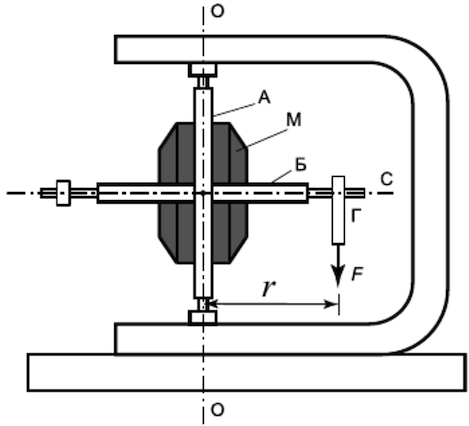
\includegraphics[width=2.5in]{gy1.png}  \\ Рис 1: Гироскоп 
    \end{center}

    \begin{center} 
        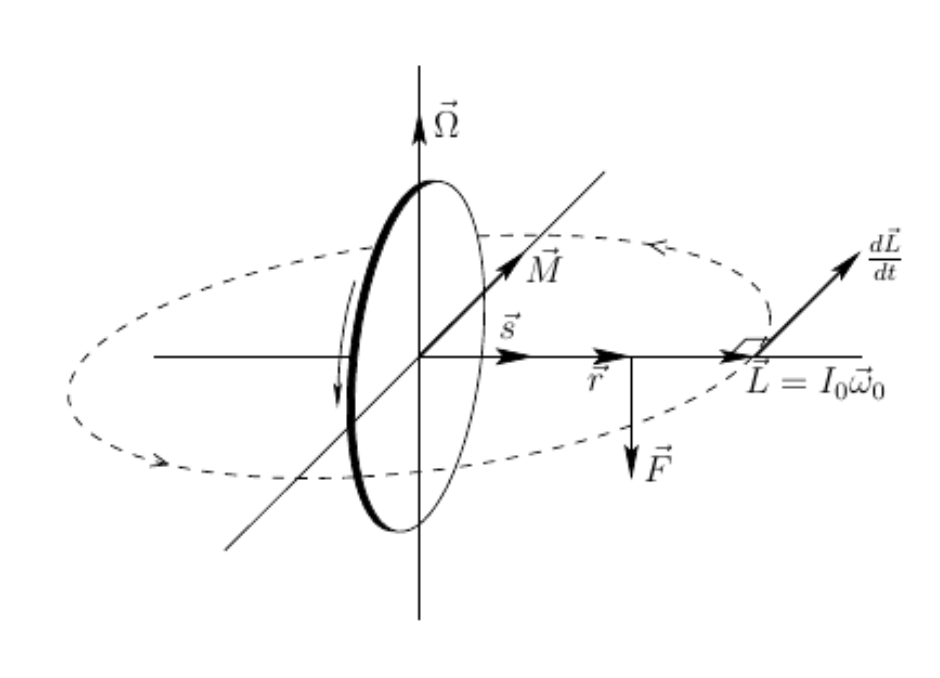
\includegraphics[width=2.5in]{gy2.png} \\ Рис 2: Вынужденная прециссия гироскопа
    \end{center}


    Движение осесимметричного тела удобно разбить на две составляющие   выделить из вектора полной угловой скорости $\vec{\omega}$ угловую скорость вращения оси симметрии $\vec{\Omega}$ (угловая скорость прециссии) , которую обычно называют угловой скоростью прецессии, и $\vec{\omega_0}$   угловую скорость  собственного  вращения:
    \begin{equation}
        \vec{\omega} = \vec{\omega_0} + \vec{\Omega} 
    \end{equation}


    В зависимости от того, приложены или нет к гироскопу какие-либо внешние силы, различают два типа его движения:
    \begin{enumerate}
        \item Если момент внешних сил равен нулю ($\vec{M} = 0$), то  сохраняется момент импульса системы: $\vec{L} = const$.
    
    Если раскрутить гироскоп исходно только вокруг своейоси (т. е. $\vec{\Omega} = 0$), то вектор угловой скорости $\vec{\omega_0}$ также должен оставаться неизменным по модулю и направлению, а следовательно, и ось гироскопа ($\vec{s}$) должна сохранять свою ориентацию в пространстве при любом перемещении центра масс системы.
    \item Если же приложить к исходно уравновешенному гироскопу внешнюю силу с ненулевым моментом , то гироскоп придёт в движение, определяемое уравнением:
    \begin{equation}
        \vec{\Omega} \times \vec{L} = \vec{M}    
    \end{equation}

    \textbf{Ход работы:}
        \item По реакции гироскопа определим, в какую сторону вращается ротор. Совпадает с направлением гироскопа, изображенного на Рис. 2.

        \item Определим момент инерции ротора гироскопа по формуле
    
    $$I_0 = I_\text{ц} \frac{T_0^2}{T_\text{ц}^2},$$
    где $I_\text{ц} = \frac{mr^2}{2}$ , $T_\text{ц}$ и $T_0$ - периоды колебаний на проволочном подвесе цилиндра и ротора гироскопа соответственно. \\
    Проведем необходимые измерения:
    $t_6 = $ [28.20 , 28.28 , 28.37 , 28.50 , 28.40 , 28.59] c - 6 измерений времени 6-ти полных колебаний ротора. \\
    $T_{\text{0}} = 4.73$ , $\sigma_0 = 0.02$ , $\varepsilon_0 \approx 0.005 = 0.5\%$ - относительная погрешность. \\ \\
    \underline{Параметры цилиндра:} \\
    $m_{\text{ц}} = 1617.7$ g - масса\\
    $d_{\text{ц}} = 7.8$ cm - диаметр \\
    $t_{\text{ц}} = $ [35.97 , 36.06 , 36.25 , 36.03 , 36.25 , 36.10] c  - время 6-ти полных колебаний цилиндра.\\
    $T_{\text{ц}} = 6.02$ c \\ 
    $\sigma_{\text{ц}} = 0.02$ , 
    $\varepsilon_{\text{ц}} \approx 0.003 = 0.3 \%$

    Получим $I_{\text{ц}}=12.30 \cdot 10^{-4}$ $\rightarrow$ $I_{0} \approx 7.6 \cdot 10^{-4}$  $kg/m^2$  \\
    $$\left(\frac{\sigma_{I_0}}{I_0}\right)^2 
    = \left(\frac{\sigma_{m}}{m}\right)^2
    + 4\left(\frac{\sigma_{r}}{r}\right)^2
    + 4\left(\frac{\sigma_{T_0}}{T_0}\right)^2
    + 4\left(\frac{\sigma_{T_\text{ц}}}{T_\text{ц}}\right)^2$$
    
    $\sigma_{I_0} = 0.2 \cdot 10^{-4} \text{ кг}\cdot\text{м}^2$
    \item
    \underline{Параметры установки:} \\ 
        $R = 18.6$ см - радиус для измерения вертикального угла отклонения \\
        $r = 12.3$ см - плечо силы \\

        Результаты измерения количества полных оборотов и вертикального отклонения в зависимости от веса грузов:
                    \begin{center}
                    \begin{tabular}{|c|c|c|c|c|c|c|c|c|c|}
                        \hline
                            $t_tr$ , min & 2.30 & 2.36 & 2.11 & 1.48 & 2.51 & 2.18 & 2.47 & 2.10 & 3.28 \\
                            \hline
                            $n_\text{оборотов}$ & 1 &1 &1 &1&2&2&3&3&4 \\
                            \hline
                            $m$ , g  & 60 &76&93&116&141&173&215&268&335 \\
                            \hline
                            $\Delta h$ , cm & 3.9& 2.6& 2.0& 1.7& 3.1& 2.2& 2.5& 2.1& 1.3 \\
                            \hline
                    \end{tabular}
                    \end{center}
    \item Найдем угловую скорость прециссии как :
    $$\Omega = \frac{2\pi n}{t} = \frac{2\pi}{T}$$
    
    Ошибка $\Omega$:
    $$ \sigma_{\Omega} = 2 \pi \Omega \left(\frac{\sigma_{T}}{T}\right)$$

    \begin{center} 
        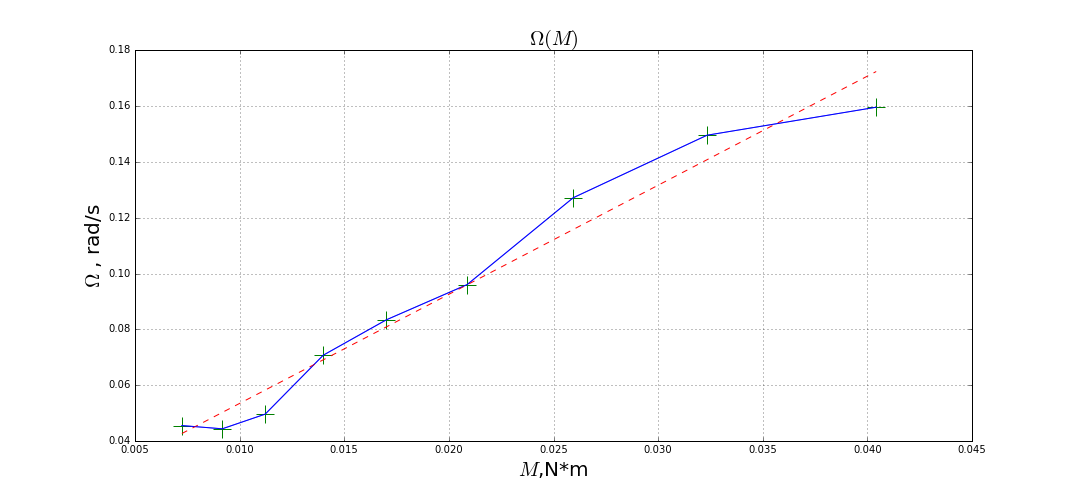
\includegraphics[width=6.5in]{graph.png} 

        $y = kx + b$ , $k \approx 3.91$  , $b \approx 0.014$ , $\sigma_k \approx 0.23$ , $\sigma_b \approx 0.003$\\
    \end{center}

    
    \end{enumerate}


\end{document}